\documentclass[border=5mm]{standalone}
\usepackage{tikz}
\usepackage{pgfplots}
\usepackage{xcolor}
\pgfplotsset{compat=1.18}

% Definir colores exactos
\definecolor{celeste}{RGB}{0,206,209}
\definecolor{naranja}{RGB}{255,140,0}
\definecolor{siena}{RGB}{205,133,63}

\begin{document}
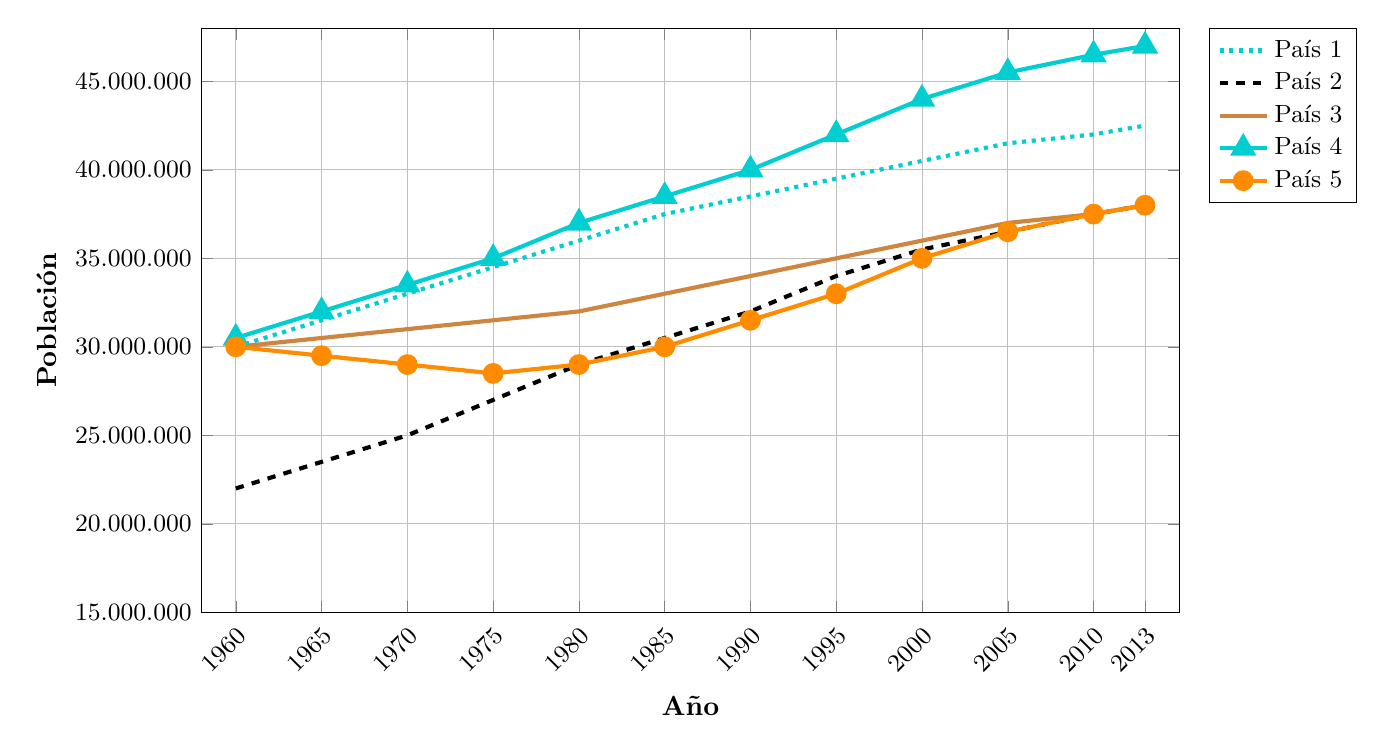
\begin{tikzpicture}
\begin{axis}[
    width=14cm,
    height=9cm,
    xlabel={Año},
    ylabel={Población},
    xmin=1958, xmax=2015,
    ymin=15000000, ymax=48000000,
    xtick={1960,1965,1970,1975,1980,1985,1990,1995,2000,2005,2010,2013},
    xticklabel style={font=\small, rotate=45, anchor=north east, /pgf/number format/1000 sep={}},
    ytick={15000000,20000000,25000000,30000000,35000000,40000000,45000000},
    yticklabels={15.000.000,20.000.000,25.000.000,30.000.000,35.000.000,40.000.000,45.000.000},
    scaled y ticks=false,
    grid=both,
    grid style={line width=0.3pt, draw=gray!50},
    legend pos=outer north east,
    legend style={font=\small, cells={anchor=west}},
    tick label style={font=\small},
    xlabel style={font=\bfseries},
    ylabel style={font=\bfseries}
]

% País 1 - Línea punteada celeste (sin marcadores)
\addplot[color=celeste, dotted, line width=1.5pt, mark=none] coordinates {
    (1960,30000000) (1965,31500000) (1970,33000000) (1975,34500000)
    (1980,36000000) (1985,37500000) (1990,38500000) (1995,39500000)
    (2000,40500000) (2005,41500000) (2010,42000000) (2013,42500000)
};
\addlegendentry{País 1}

% País 2 - Línea discontinua negra (sin marcadores)
\addplot[color=black, dashed, line width=1.5pt, mark=none] coordinates {
    (1960,22000000) (1965,23500000) (1970,25000000) (1975,27000000)
    (1980,29000000) (1985,30500000) (1990,32000000) (1995,34000000)
    (2000,35500000) (2005,36500000) (2010,37500000) (2013,38000000)
};
\addlegendentry{País 2}

% País 3 - Línea sólida marrón/siena (sin marcadores)
\addplot[color=siena, solid, line width=1.5pt, mark=none] coordinates {
    (1960,30000000) (1965,30500000) (1970,31000000) (1975,31500000)
    (1980,32000000) (1985,33000000) (1990,34000000) (1995,35000000)
    (2000,36000000) (2005,37000000) (2010,37500000) (2013,38000000)
};
\addlegendentry{País 3}

% País 4 - Línea celeste con triángulos rellenos
\addplot[color=celeste, solid, line width=1.5pt, mark=triangle*, mark size=4pt, mark options={fill=celeste}] coordinates {
    (1960,30500000) (1965,32000000) (1970,33500000) (1975,35000000)
    (1980,37000000) (1985,38500000) (1990,40000000) (1995,42000000)
    (2000,44000000) (2005,45500000) (2010,46500000) (2013,47000000)
};
\addlegendentry{País 4}

% País 5 - Línea naranja con círculos rellenos
\addplot[color=naranja, solid, line width=1.5pt, mark=*, mark size=3pt, mark options={fill=naranja}] coordinates {
    (1960,30000000) (1965,29500000) (1970,29000000) (1975,28500000)
    (1980,29000000) (1985,30000000) (1990,31500000) (1995,33000000)
    (2000,35000000) (2005,36500000) (2010,37500000) (2013,38000000)
};
\addlegendentry{País 5}

\end{axis}
\end{tikzpicture}
\end{document}
